\documentclass[11pt]{article}
\usepackage[round,comma,authoryear]{natbib}
\usepackage{fullpage}
\usepackage{authblk}
\usepackage{graphicx}
\usepackage{booktabs}
\usepackage{amsmath}

\usepackage[newfloat]{minted}
\usepackage{tcolorbox}
\usepackage{etoolbox}
\BeforeBeginEnvironment{minted}{\begin{tcolorbox}}
\AfterEndEnvironment{minted}{\end{tcolorbox}}
\usepackage{url}
\usepackage{fancyvrb}
\usepackage{caption}
\newenvironment{code}{\captionsetup{type=listing}\centering}{}
\SetupFloatingEnvironment{listing}{name=Demographic Model}
% can either input code directly in a minted environment
% or input from a source file using \inputminted

% local definitions
\newcommand{\ms}[0]{\texttt{ms}}
\newcommand{\msprime}[0]{\texttt{msprime}}
\newcommand{\stdpopsim}[0]{\texttt{stdpopsim}}
\newcommand{\demes}[0]{\texttt{demes}}
\newcommand{\demesdraw}[0]{\texttt{demesdraw}}
\newcommand{\Demes}[0]{\texttt{Demes}}
\newcommand{\moments}[0]{\texttt{moments}}
\newcommand{\dadi}[0]{\texttt{$\partial$a$\partial$i}}
\newcommand{\fwdpy}[0]{\texttt{fwdpy11}}
\newcommand{\slim}[0]{\texttt{SLiM}}
\newcommand{\gadma}[0]{\texttt{GADMA}}

\newcommand{\aprcomment}[1]{{\textcolor{blue}{APR: #1}}}
\newcommand{\jkcomment}[1]{{\textcolor{red}{JK: #1}}}
\newcommand{\ggcomment}[1]{{\textcolor{yellow!60!red}{GG: #1}}}
\newcommand{\krtcomment}[1]{{\textcolor{purple}{KRT: #1}}}
\newcommand{\mhcomment}[1]{{\textcolor{cyan}{MH: #1}}}

\usepackage{catchfile}
\begin{filecontents*}{software-table.tex}
\end{filecontents*}

\begin{document}

\title{Demes: a specification for interchanging complex demography}
% First authors
\author[1,$\star$]{Graham Gower}
\author[2,$\star$]{Aaron P. Ragsdale}

% Authors: please add your name and affiliation here, in alphabetical order.
% Second Authors
\author[3]{Ryan N. Gutenkunst}
\author[4]{Matthew Hartfield}
\author[5]{Ekaterina Noskova}
\author[3]{Travis J. Struck}
%Senior Authors
\author[6,$\dagger$,$\aleph$]{Jerome Kelleher}
\author[7,$\dagger$]{Kevin R. Thornton}

\affil[1]{Lundbeck GeoGenetics Centre, Globe Institute, University of Copenhagen}
\affil[2]{Department of Integrative Biology, University of Wisconsin--Madison}
\affil[3]{Department of Molecular and Cellular Biology, University of Arizona}
\affil[4]{Institute of Evolutionary Biology, The University of Edinburgh}
\affil[5]{Computer Technologies Laboratory, ITMO University}
\affil[6]{Big Data Institute, Li Ka Shing Centre for Health Information and
    Discovery, University of Oxford}
\affil[7]{Ecology and Evolutionary Biology, University of California at Irvine}

\affil[$\star$]{Denotes shared first authorship, listed alphabetically}
\affil[$\dagger$]{Denotes shared senior authorship, listed alphabetically}
\affil[$\aleph$]{Denotes corresponding author}


\maketitle

\begin{abstract}
Understanding the demographic history of populations is a
key goal in population genetics, and with improving methods
and data, ever more complex models are being estimated.
Demographic models of current interest
typically consist of a set of discrete populations,
their sizes and growth rates, and continuous and pulse migrations
between those populations over a number of epochs, which can require
dozens of parameters to fully describe. There is currently
no standard format to define such models, significantly
hampering  progress in the field. In particular, the important
task of translating the model descriptions in published
work into input suitable for population genetic simulators is labour intensive
and error prone.
We propose the Demes data model and file format,
built on widely used technologies,
to alleviate these issues. Demes provides a well-defined and unambiguous
graphical model of populations and their properties that is straightforward to
implement in software, and a text file format that is designed for
simplicity and clarity.
We provide thoroughly tested implementations of Demes parsers in Python
and C, and showcase initial support in a number of simulators and inference
methods.
\end{abstract}


\section*{Introduction}

The ever-increasing amount of genetic sequencing data from genetically and
geographically diverse species and populations has allowed us to infer complex
demography and study life history at fine scales.
An integral component to such population genetics studies is simulation.
Software to either simulate whole genome
sequences~\citep{thornton2014cpp,thornton2019-nu,staab2015scrm,baumdicker2021-iu,kelleher2016efficient,haller2019slim}
or informative summary statistics of
diversity~\citep{gutenkunst2009inferring,kamm2017efficient,jouganous2017inferring}
have enabled the increasing complexity of genomic studies, with several software
packages capable handling large sample sizes, many interacting populations, and
deviations from panmictic random-mating assumptions.
This ability to infer and simulate such complex demographic scenarios, however,
has highlighted a major shortcoming in community standards.
The fragmented landscape of different approaches to describing demographic
models makes it difficult to compare inferences made by different methods
and to reliably simulate from previously inferred models.

Inference methods for demography usually output a set of
text files which describe the inferred model,
and nearly all methods use different file formats.
Inference results are typically reported in publications
via a combination of visual depiction,
a list of key parameters in tabular form and a discussion within the text.
Unfortunately these descriptions are often ambiguous, and
implementing the precise model inferred for later simulation
is at best tedious and error prone~\citep{ragsdale2020lessons}
and occasionally impossible because of missing information. \mhcomment{Maybe add a short, concrete example to convince readers of the problem?}
%\aprcomment{This feels tangential - maybe discussion}
%The \stdpopsim\ project is a community-maintained catalog of species
%information and demographic models designed to provide standardised
%population genetic simulations~\citep{adrion2020community}.
%The development process for adding demographic models to
%\stdpopsim\ tries to avoid errors in model implementation by requiring two
%independent implementations of each model
%to be equivalent. While this process is
%robust and has uncovered both significant
%errors~\citep{ragsdale2020lessons} and ambiguities in
%published models, it is labour intensive.
Instead, it would be far better if published results were reported
in an unambiguous standardised format that could be provided
directly as input to simulators.

Simulation is a core tool in population genetics, and a
many methods have been developed over the past three
decades~\citep{carvajal2008simulation,liu2008survey,
arenas2012simulation,yuan2012overview,hoban2012computer}.
Simulations are based on highly idealised population models,
and one of the key uses of inferred demographic histories
is to make simulations more realistic.
Simulation methods take three broad approaches to specifying
the demographic model to simulate,
using either a command line
interface~\citep[e.g.][]{hudson2002generating,kern2016discoal},
a custom input file
format~\citep[e.g.][]{guillaume2006nemo,excoffier2011fastsimcoal,shlyakhter2014cosi2},
or an Application Programming Interface (API) to allow
models be defined programmatically~\citep[e.g.][]{
thornton2014cpp,thornton2019-nu,baumdicker2021-iu,kelleher2016efficient,becheler2019quetzal,haller2019slim}.
Command line interfaces are a concise way of expressing
demographic models, and the syntax defined by \ms~\citep{hudson2002generating}
is used by a number of different
simulators~\citep[e.g.][]{ewing2010msms,chen2009fast,staab2015scrm},
and the POPDemog visualisation software~\citep{zhou2018popdemog}.
However, this conciseness means that models of even intermediate complexity
are difficult for humans to understand, making errors highly likely.
Input parameter file formats for simulators allow the model specification
to be less terse and allow for documentation in the form of comments.
However, there is no standard format shared across simulators,
and the details of the demographic models are not separated
from other simulation parameters.
The APIs used by individual simulators to define demographic models are also
not appropriate as an interchange standard because of the dependency on both
the programming language involved,
and the specific details of the simulator in question.

Here we present ``Demes'', a data model and file format specification for
complex demographic models developed by the
PopSim Consortium~\citep{adrion2020community}.
The Demes data model precisely defines the sizes and relationships
of populations, and it provides a way to explicitly encode the
information relevant to demography while avoiding repetition.
This data model is implemented in the widely used YAML
format~\citep{ben2009yaml}, which provides a good balance between human
and machine readability.
The specification precisely defines the required behaviour of implementations,
ensuring that there is no ambiguity of interpretation, and includes both a
reference implementation and an extensive suite of test examples and their
expected output.
The initial software ecosystem includes high-quality Python
and C parser implementations, as well as utilities for verification and
visualisation of Demes models, and has been implemented in several popular
inference and simulation methods (Table~\ref{tab:software}).
We hope that this data model and file format will be widely adopted
by the community, such that users can expect to simulate directly
from inferred models with little programming effort.


\section*{Demes}

The design of Demes is a balance between two partially competing requirements:
that (a) models should be easy for humans to understand and manipulate;
and (b) software processing Demes models should be provided with an unambiguous
representation that is straightforward to process.
For efficiency of understanding and avoidance of model specification error,
we require a data representation without redundancy (i.e., repetition of values).
However, for the simplicity of software working with the Demes model
(and the avoidance of programming error, or divergence in
interpretations of the specification) it is preferable to have an explicit
representation, in which all relevant values are readily available.
Thus, Demes is composed of three entities: the high-level, human-readable
model specification; the low-level, fully-qualified model
specification; and the parser, which is responsible for transforming the former
into the latter.

Below we provide a brief overview of the population genetics models
that Demes supports and the components of the Demes infrastructure.
We then highlight an example usage, including visualization and simulation
of a multi-population demographic model.
Detailed descriptions of the population genetics model, parsers, scope, and
additional examples are given in the Appendix.

\CatchFileDef{\softwaretable}{software-table.tex}{}
\renewcommand{\arraystretch}{1.5}
\begin{table}
    \begin{center}
        \begin{tabular}{lp{12cm}}
            \softwaretable
        \end{tabular}
    \end{center}
    \caption{
        \label{tab:software}
        \textbf{Software support for Demes.}
        We have included software infrastructure developed
        for working with Demes models (parsing, validation,
        visualisation, etc) as well as all known downstream 
        software that implements the specification,
        at the time of writing.
    }
\end{table}

\subsection*{Population genetics model}

Demographic models consist of one or more populations (or ``demes'') defined
by their size histories and the time intervals of their existence.
Individuals can move between populations based on their ancestor-descendant
relationships (i.e., the topology) or by continuous or discrete migration events.
The deomgraphic model itself omits information about genome biology, such as
genome size and architecture, ploidy, and mutation and recombination rates.
It also omits any information about selection operating within populations.
Within populations, allele-frequency dynamics are assumed to
follow the Wright-Fisher model, so that generations are discrete and
non-overlapping and population sizes are independent of mean fitness
(i.e., ``soft'' selection~\citep{christiansen1975hard}).
While these restrictions preclude some population-genetic scenarios of
interest, such as continuous spatial structure
\aprcomment{citations here, and revisit} or
\aprcomment{stochastic carrying-capacity models, or something like that},
many current forwards- and backwards-in-time simulation software
make these same assumptions, so that Demes is relevant to a range of
widely-used simulators.
\jkcomment{I guess these are also the basic assumptions also shared by
inference methods, which is important. Mabye another sentence here making this
explicit, and listing a few different types of inference methods and giving
citations? This is critical - we want to establish that Demes is the
"middleware" between the inference methods and the simulators, and captures the
basic assumptions made by them all.}
In Appendix~\ref{sec:appendix-pop-gen-model}, we expand on these concepts
and provide more details on the population genetics models supported by Demes.

\subsection*{High-level specification}

The high-level description of Demes models is focused on efficient human
understanding and avoiding errors.
We have adopted the widely used YAML format~\citep{ben2009yaml} as the
primary interface for writing and interchanging demographic models
(see Appendix~\ref{sec:appendix-spec} for details about our choice of
YAML formatting for demographic models).
Demographic models written in YAML format provide information about global
features of the model (such as time units and generation times),
populations (as ``demes'') and their existence intervals (as ``epochs''),
and gene flow between populations
(as continuous ``migrations'' or instantaneous ``pulse'' events)
(e.g., Figures~\ref{fig:showcase}~and~\ref{fig:IM}).
The high-level Demes specification encourages human understanding by avoiding
redundancy in the description where possible and by providing a mechanism for
specifying default values that are inherited hierarchically.

\subsection*{Parsers}

While the high-level specification is designed for human readability and
conciseness, the underlying data model suitable for software implementation
is redundant and exhaustive. 
Translation from the high-level specification to the low-level data model
requires resolving heierarchically-defined default values and verifying
relationships between populations and the validity of specified parameter
values.
Because this translation and validation requires significant
programming effort, we define a standard software entity as part of the
specification to perform this task (the parser),
which is intended to be shared by programs that support Demes as an input.
By having relatively few high-quality Demes parsers available as libraries
(ideally one per programming language), we ensure consistency across simulation
software in their implementation of Demes-specified models.
We provide a reference implementation written in Python to resolve any
potential ambiguities and to provide a helpful template for other
implementations, as well as an extensive test suite of examples and the
expected outputs.
In addition, we have high-quality parser implementations in the Python and
C languages (published under liberal open source licences), providing a
solid foundation for the software ecosystem (Table~\ref{tab:software}).

\aprcomment{redundancies with Appendix - that could be expanded and reworked a bit}

\subsection*{The scope of Demes}

The Demes specification is static by design -- we wish to unambiguously
describe a demographic model with a concrete set of parameters.
This simplicity means that we cannot directly specify parameter distributions
or estimated confidence intervals for those parameters.
While it is not difficult to imagine extending the specification in ways that
would allow this (Appendix~\ref{sec:appendix-scope}), it is not immediately
clear that the benefits are worth the increased parser complexity.

Demes is also designed to interface with a large number of simulation and
inference methods, so we have restricted the specification to only
describe demographic features at the population level.
The underlying discrete demographic structure is the common thread connecting
many widely-used population genetic methods, so we have omitted many
features of the underlying genome biology (as described above, and in
Appendix~\ref{sec:appendix-scope}).

\section*{Application: simulation using Demes}

\aprcomment{Need a paragraph or two here, extolling the virtues of simulation with demes}

\begin{itemize}
    \item Multi-population model with migrations and/or pulses
    \item Demesdraw
    \item msprime simulation
    \item moments simulation
    \item Compare SFS in each population
    \item The input YAML file should go in the Appendix
\end{itemize}

\begin{figure}[tb!]
    \centering
    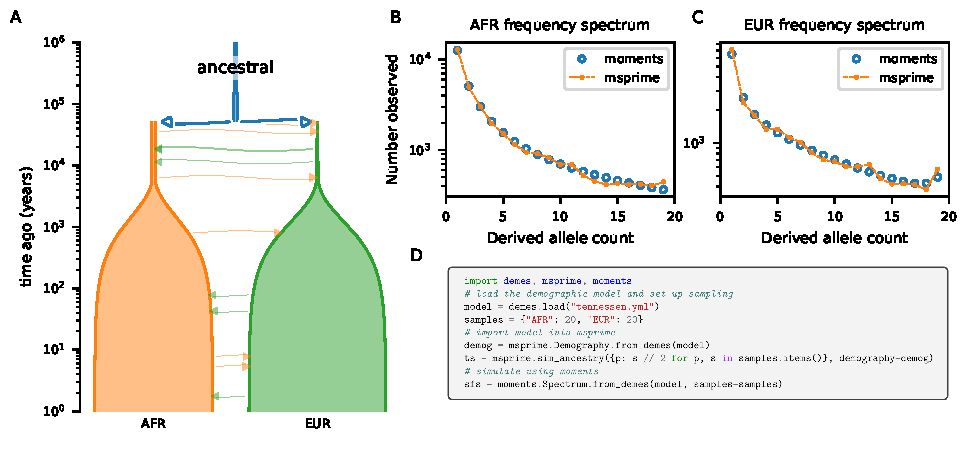
\includegraphics{fig/showcase}
    \caption{
        \textbf{Illustration and simulation using Demes.}
        (A)
        Using an inferred demographic model from \citet{tennessen2012evolution}
        specified as a YAML in Demes format (Figure~\ref{fig:tennessen}), we
        use \demesdraw\ to visualize the demographic model.
        We then use \msprime\ to simulate genomic data for 20 genome copies
        sampled from the two contemporary populations, and we use \moments\
        to compute the expected joint site-frequency spectrum for the same
        sample sizes (Figure~\ref{fig:tennessen-simulation}).
        (B, C) We compare the single-population SFS in each population, showing
        agreement between the simulation methods.
        (D) Code snippets of the interactions between \demes\ and the simulation
        software. An extended script to compute the SFS shown in (B) and (C) is
        given in Figure~\ref{fig:tennessen-simulation}.
        \aprcomment{There may be a better model to use here -- the massive
        exponential growth really makes the rest of the history hard to see.}
    }
    \label{fig:showcase}
\end{figure}

\section*{Discussion}

The difficulty of describing complex demographic models
for population genetic simulations has long been acknowledged
~\citep[][e.g.]{antao2007modeler4simcoal2}, % jk - any older refs for this?
and a number of different methods have been proposed to
make such simulations more accessible and less error prone.
Several Graphical User Interface (GUI) and visualisation
methods have been developed, which greatly facilitate
interpretation~\citep{mailund2005coasim,antao2007modeler4simcoal2,
ewing2010msms,zhou2018popdemog}. However, these methods
currently have little traction as they are all either directly coupled
to an internal simulation method or to the specific syntax
of a given simulator. Another approach that has been taken to
simplify running such simulations is to provide an API in a
scripting language such as Python or R, providing a flexible
interface either to a built-in simulation
engine~\citep{thornton2014cpp,thornton2019-nu,baumdicker2021-iu,kelleher2016efficient,haller2017flexible}
% jk: are/were there other simulation frontends out there?
or as a front end for other simulators~\citep{staab2016coala}.
While APIs have many advantages and have grown in popularity in
recent years, the demographic model descriptions are tied
to the details of both the underlying simulation engines
and the programming language in question.

Stable and healthy software ecosystems require standard interchange
formats, allowing for the development of high-quality and long-lasting
tools that produce and consume the standard.
Demographic models are a key part of population genetics research,
and to date the transfer of inferred models to downstream simulations
has been ad-hoc, and conversions between the many different ways
of expressing such models is both labour intensive and fraught with errors.
The proposed Demes standard is an attempt to bridge this gap
between inference and simulation, and also to provide the foundations
for a sustainable ecosystem of tools built around this data model.
Table~\ref{tab:software} shows some initial infrastructure that we have
built as part of developing Demes, but many other useful tools
can be envisaged that consume, transform, or produce this format.

Reproducibility is a significant problem throughout the
sciences~\citep{baker20161} and various measures have been
proposed to increase the likelihood of researchers being
able to replicate results in the
literature~\citep{munafo2017manifesto}. The most basic requirement
for reproducibility is that we must be able to state precisely what
the result in question is. The lack of standardisation in how
complex demographic models are communicated today, and the lack of
precision in the published model descriptions means that it is difficult
to replicate analyses, or reproduce those models for later simulation.
Thus, we hope that the Demes standard introduced here will be widely adopted
by simulation and inference methods and be used for reporting results in
publications, either as supplemental material or uploaded to a data
repository in Demes format.

\krtcomment{Here, we should say something about other models that people may wish to implement within the demes
framework.}


\bibliographystyle{genetics}
\bibliography{paper}

\renewcommand{\thefigure}{A\arabic{figure}}
\renewcommand{\thetable}{A\arabic{table}}
\renewcommand{\theequation}{A\arabic{equation}}
\renewcommand{\thesection}{A\arabic{section}}
\setcounter{figure}{0}
\setcounter{table}{0}
\setcounter{equation}{0}

\section*{Appendix}

The Demes specification is a formal data model for describing
the properties of populations over time,
along with some metadata and provenance information.
The data model is based on the ubiquitous JSON~\citep{bray2017javascript}
standard, and the structure is formally defined using
JSON Schema~\citep{wright2020json}.
The Demes JSON schema rigorously defines the data model,
specifying the hierarchical structure and the properties that are allowed in different
contexts along with their types and permissible ranges.
This schema, and its accompanying documentation,
fully describe the entities in the model and their
relationships and the required behaviour of implementations.
Since the schema is definitive, we will not recapitulate the details
here, but instead focus on the high level properties of the model and
the rationale behind key design decisions.

Below, we detail
\begin{itemize}
    \item The population genetics model in Section~\ref{sec:appendix-pop-gen-model}
    \item The high-level model specification in Section~\ref{sec:appendix-spec}
    \item The desired behaviour of Demes-format parsers in Section~\ref{sec:appendix-parsers}
    \item And the intended scope of Demes in Section~\ref{sec:appendix-scope}
\end{itemize}

\section{Population genetics model details}\label{sec:appendix-pop-gen-model}

In Demes, demographic models consist of one or more interacting populations,
or ``demes'', by which we mean a grouping of individuals that is convenient
for modelling \citep{gilmour_demes_1939,gilmour_deme_1955}.
To avoid confusion with the name of the specification itself we will
use the term ``population'' in this discussion, with the understanding that the
terms are interchangeable for our purposes.
A population is defined as some collection of individuals that exists for
some period of time, and has a well-defined size (i.e., number of individuals)
during that time period. Individuals can move between populations
either through ancestor-descendant relationships between the populations,
or through processes of continuous or pulse migration.
No other properties of the populations are specified in the model:
we are concerned only with defining the populations, their sizes, and the
movement of individuals between those populations.

Population and event times are written as units in the past, so that time zero
corresponds to the final generation or ``now'', and event times in the past are
values greater than zero with larger values for events that occur in the more
distant past. By having time units increase into the past, we avoid the need to
choose an arbitrary point in history as ``time zero'', so that instead zero
refers to ``now'' or the final generation of a simulation. A natural
specification for time units is in generations, although other time units are
permitted, such as years, accompanied by the generation time.

Population sizes are given as numbers of individuals, and details
such as ploidy levels are considered external to the model.
We therefore focus on the number of individuals as opposed to the number of genomes.
Sizes and mating system details are specified for each population within
epochs.
Epochs are contiguous time intervals that define
the existence interval of the population. Each epoch specifies the population size
over that interval, which can be a constant value or function defined by start
and end sizes that must remain positive.

\krtcomment{The paragraph(s) below subsume(s)/replace(s) some of what appears in later pargraphs.
	I'm not making an attempt yet to revise that later content--I think other authors should
	weigh in.}

\krtcomment{Aaron -- I have perhaps over-simplified the description of marginal allele frequency dynamics?}

Within a population, we implicitly assume that allele frequency dynamics can
be described by the Wright-Fisher model.  Briefly, generations are non-overlapping (all parents
reproduce and die simultaneously) and the expected frequency (at birth) of the $i^{th}$ allele currently at frequency $p_i$
one generation in the next generation is $p_iw_i/\bar{w}$, where $w_i$ and $\bar{w}$ are the marginal and
mean fitnesses, respectively, properly weighted according to ancestry proportions. In this framework,
a forward-time simulation of finite populations is equivalent to multinomial sampling of allele frequencies each
generation (\citet[][pp 29-31]{burger2000-ul}, \citet[][pp 179-181]{crowkimura1970})
and a backwards-time (coalescent) simulation follows the approximations described in \cite[][chapter 3]{wakeley2008-hd}.
Further, this model assumes "soft" selection \citep{christiansen1975hard}, meaning that the dynamics of population sizes
changes are \textit{independent} of the details of individual fitnesses.
In the \texttt{Discussion}, we discuss alternative models compatible with this framework and outline the expectations for tools implementing
them.
A plethora of forwards and backwards time simulators currently implement this model (REFS).
Each has their own unique method of specifying the details of selection and demography.
The goal of \Demes\ is to provide a common method for the latter task.  

\krtcomment{We need to revisit the paragraph(s) below.  We do not assume individuals are exchangeable, because we do not
	require that all individuals have the same fitness. See, e.g., p 60 of Wakeley for why fitness == exchangeability
	and why that is required for the standard coalescent.}
\mhcomment{The `exchangeability' assumption also breaks down under different reproductive modes, since the sampling of the alleles affects coalescent times. For example, in a highly selfing species the coalescent time for two different alleles within an individual is much lower than two alleles from different individuals. I've tried to rewrite the below paragraph to update and clarify the reproduction parameters in line with the discussions on Github. Finally, 'rates' imply events occur as Poisson-like processes over continuous time, whereas the values used here instead define the \emph{fraction} of reproductions of each type. Shall we rename to selfing/clonal `fractions', or would that mess up the rest of the schema too much?}

Each population has a selfing rate and cloning rate assigned to it, where each denotes the probability that offspring are generated from one generation to the next by either self-fertilisation or cloning of an individual. More specifically, denote the clonal rate by $\sigma$ and the selfing rate by $S$. In each population a proportion of offspring $\sigma$ reproduce clonally, while $1-\sigma$ reproduce sexually. Within the sexually--reproducing offspring, $S$ were born via self--fertilisation while the rest were outcrossed. Hence $S$ and $\sigma$ can take any value between zero and one, but do not have to sum to one. See \citet{hartfield2016facsexcoal} for more details of the mathematical properties of these rates in a coalescent context. \mhcomment{If requested I can quickly draw up a schematic diagram to illustrate these partitions.} Note that even if $S$, $\sigma$ are set to zero then some residual selfing can occur due to sampling in the Wright--Fisher model.

%Within a population, individuals are assumed to be exchangeable, but there are
%also parameters for nonrandom mating, such as selfing or cloning rates, which
%give the probability that offspring are generated from one generation to the
%next by self-fertilisation or cloning of an individual. Cloning and selfing
%rates can take any value between zero and one, and if both are specified then
%the selfing rate is the probability an offspring is generated through
%self-fertilisation given it was produced sexually (i.e. with probability one
%minus the cloning rate). 

We omit any details regarding selection.
Thus, the history of population size changes does not depend on mean fitnesses within
a population nor on differences in mean fitness between populations.
This indepedence of population size and
selection is often called ``soft" selection \citep{christiansen1975hard}.

List of thoughts to turn into a paragraph:

\begin{enumerate}
    \item Selection parameters may be arbitrarily complex.  Different fitness effects in different demes.
          Variation over time.  Etc..
          The specification would become unwieldy and perhaps limiting.
    \item By allowing selfing and cloning, we allow many "standard" models to be considered with "no or little"
          extra effort.
    \item However, by parameterising selfing and cloning as we have, we are assuming that these properties of
          populations at given times can be specified independently from the genetics.
          In other words, mutations that cause selfing to "come and go" are not considered.
          However, consuming software is free to ignore these parameters and model the genetics within
          the framework of a soft selection model.
    \item We don't view these as limitations. Rather, this is what most people are doing most of the time.
          Just now we can finally try to do this part w/fewer errors.
\end{enumerate}


\aprcomment{If selection is placed on top of the demographic model, this implies
that we are living in a soft selection world. Though sizes could just as easily
be interpreted as carrying capacities in a hard selection model.}
\krtcomment{We are firmly in the soft selection world here.  The connection to hard selection
requires some other strong assumptions that will sometimes be met, and sometimes not.
For example, if the mean fitnesses are approximately equal across demes, then a hard selection
model could be similar to a soft selection model.  Relevant literature to dig up: Felsenstein's review,
which will lead to other stuff.}

\jkcomment{More detail here. Also, why only selfing and cloning, why not selection
coefficients and whatnot?}
\krtcomment{Selection is a can of worms: scaling of diploid genotype fitnesses will differ between tools.
The possibility of "GxE" ("different s for same genotype in different demes") can lead to quadratic complexity.}

A population may have one
or more ancestors, which are other populations that exist at the population's
start time. If one ancestor is specified, the first generation is constructed
by randomly sampling parents from the ancestral population to contribute to
offspring in the newly generated population. If more than one ancestor is
specified, the proportions of ancestry from each contributing population must
be provided, and those proportions must sum to one. In this case, parents are
chosen randomly from each ancestral population with probability given by those
proportions.

Finally, individuals in a population may have parents from a different
population through migrations. These can be defined as continuous migration
rates over time intervals for which populations coexist or through
instantaneous (or pulse) migration events at a given time. Continuous migration
rates are defined as the probability that parents in the ``destination''
population are chosen from the ``source'' population.
On the other hand, pulse
migration events specify the instantaneous replacement of a given fraction of
individuals in a destination population by individuals with parents from a
source population.

This model is, by design, very limited. We do not specify any details of
individuals or of the processes that happen \emph{within} populations,
because such details are necessarily complicated, vary greatly by
application, and any attempt to encompass such a broad range of biological
processes is doomed to failure. An ``individual'' (i.e., a discrete
organism) is an abstraction that should have a well defined interpretation
in most cases.
This narrow focus on individuals and their groupings into populations
should ensure that the Demes standard is stable, and not subject to
continual development as more and more elaborations of basic processes
are added. We could never hope to fully encompass all the details
of every possible simulation (including ploidy,
genome sizes, recombination, mutation and gene conversion rates,
selection coefficients, and so on) and so we clearly demarcate the
% FIXME Not quite true here, we're including selfing and cloning rate
role of the specification by including \emph{none} of them.
Such details can be specified by existing mechanisms used by
simulators. If they vary according to the demography (for example,
we have different recombination maps across populations), then
we can unambiguously define these by referring to the population
identifiers and times defined by the Demes model. Rather than attempting
to embed this information \emph{in} the demographic model, we
can define it externally and refer \emph{to} the demography.

\section{High-level model specification}\label{sec:appendix-spec}

The high-level description of Demes models is focused on the efficiency of
human understanding and the avoidance of errors. We have adopted the widely
used YAML format~\citep{ben2009yaml} as the recommended means of interchanging
Demes models (see Figure~\ref{fig-example} for examples). YAML is a data
serialisation language with an emphasis on simplicity, and interoperates well
with JSON (indeed, YAML 1.2 is a superset of JSON). We chose YAML over JSON
because although JSON is an excellent format for data interchange, it is
ill-suited for human understanding or manipulation. We also considered other
declarative data exchange formats such as TOML,
but chose YAML because of equivalence with JSON,
its popularity and good software support.
Since the Demes data model is defined in JSON Schema,
however, there is no formal dependency on YAML and implementations may choose
to use JSON directly if they wish (e.g., for greater efficiency).

Structurally, the high-level Demes specification encourages human understanding
by avoiding redundancy in the description where possible and by providing a
mechanism for specifying default values that are inherited hierarchically.
Figure~\ref{fig-example} shows an example Demes model expressed in both the
high and low-level forms (both in terms of YAML syntax). For values that repeat
across fields, defaults may be used to implicitly assign default values to
fields of the given type.  A default is superseded by an explicitly provided
value if given. Other implicit values are inherited naturally following the
progression of time. For example, if an epoch \texttt{start\_size} is not
provided, it is assumed to be equal to the \texttt{end\_size} of the previous
epoch. This also means that the first epoch of each population must specify the
initial size.

\aprcomment{not sure if this is sufficient here}

\aprcomment{Need some information about defaults}

\section{Parsers}\label{sec:appendix-parsers}

The implicit value inference and default value propagation required to
fully resolve the high-level Demes model description is straightforward
to describe, but still requires significant effort to implement in
software. Moreover, there are many constraints on the data model
(for example, epoch \texttt{end\_time} values should be strictly decreasing
within a deme), which must be enforced.
It would not be reasonable to require every program that
takes Demes models as input to implement this logic, as the programming
effort would be significant (limiting adoption)
and it is likely that if there were many implementations some would differ
in their details (harming the software ecosystem).
% GG: this is currently the case for programs accepting ms command lines. E.g.
%  - MaCS interprets -es proportion as 1-proportion compared to ms.
%  - SCRM uses different options for -ema command.
We therefore define
a standard software entity as part of the specification (the parser),
which performs this task, and which can be shared by programs that
support demes as an input. By having relatively few high-quality Demes
parsers available as libraries (ideally, one per programming language),
the probability of divergences from the standard is greatly reduced.

The Demes specification precisely defines the required behaviour of parsers,
which translate the high-level specifications into unambiguous low-level
representations where all parameters have been assigned values and data
constraints have been checked. The output is formally defined as JSON, but in
practice parsers output an object model that is suitable for the particular
programming language and that can be used directly by the implementing program.
We provide a reference implementation written in Python to resolve any
potential ambiguities and to provide a helpful template for other
implementations, as well as an extensive test suite of examples and the
expected outputs. In addition, we have high-quality parser implementations in
the Python and C languages (published under liberal open source licences),
providing a solid foundation for the software ecosystem.

\aprcomment{wrapped below section about parsers to here}

\section{Scope of the specification}
\label{sec:appendix-scope}

\subsection{Static models, not parameterised models}
\label{sec:appendix-static}

\jkcomment{This section is very rough.}

% https://github.com/popsim-consortium/demes-paper/issues/3

The Demes specification is static by design---we wish to
unambiguously describe a demographic model with a concrete set
of parameters. This simplicity means that we cannot directly
specify parameter distributions or estimated confidence intervals
for those parameters. While it is not difficult to imagine extending
the specification in ways that would allow this, it's not immediately
clear that the benefits are worth the increased parser complexity.

\krtcomment{Aaron has done a bit of this non-static stuff in moments.  It may be useful to look over there?}

\ggcomment{
Possible reasons to advocate for non-static features are as follows.
\begin{enumerate}
\item Specifying prior distributions of parameters for an ABC.
\item Specifying upper and lower bounds of parameters and inter-parameter
      constraints for input to an optimisation-based inference.
\item Specifying joint distribution, or confidence intervals, for the output of
      an inference procedure.
\item Simulating from some arbitrary joint distribution that was inferred
      previously. E.g. using an ABC posterior distribution of models to
      train a neural network.
\item Extending someone else's static model to reinfer parameters,
      or add new parameters.
\end{enumerate}
}

The parameters of
demographic models are typically tightly coupled, and cases in which
distributions for different parameters can be simply described are rare.
In this situation, the simplest way to describe an estimated
distribution is to list a large number of samples from
the posterior. While writing out a large number of Demes models in
YAML format may seem inefficient, it can in fact be a compact
way to describe these distributions.
For example, consider a one-population model with piecewise-constant sizes over
20 epochs which has $\sim$~40 free parameters---the \texttt{start\_size} and
\texttt{end\_time} values for each epoch. Supposing we sample 50,000 models
from the posterior distribution, the resulting multi-document YAML file is
45~MiB.
This format compresses down to 8.4~MiB when gzipped or 6.2~MiB
when compressed with LZMA2, which is on par with an equivalent binary
representation of the free parameters
($40\times50000\times4~\text{bytes} \approx 7.6~\text{MiB}$).

Similarly, one might be interested in running simulations in which
the demographic model parameters are drawn from a distribution, e.g.,
in ABC inference~\citep{beaumont2002approximate}.
Other inference procedures based on optimising a loss function
\citep{gutenkunst2009inferring,kamm2017efficient,jouganous2017inferring}
(\ggcomment{more refs? MCMC? neural networks?})
need users to specify parameter bounds,
and possibly non-linear constraints between parameters.
Indeed, the choice of how to parameterise a model could be important for
some inference methods (e.g. absolute times versus relative times between events).

Implementing the many distributions of interest, and supporting a general
way to describe a model's free parameters, would greatly increase the
complexity of parsers, with relatively limited benefit to most users.
It's unlikely that Demes could be made sufficiently
flexible without considerable effort to implement many features of
general-purpose programming languages, such as variables, arithmetic,
and flow control.
Such use cases are therefore better served by writing model-generating
functions in an existing programming language, for example
using the Demes Python API.
To modify an existing static Demes model, perhaps to infer new parameters,
this would unfortunately require reimplementing the model.
However, there exist many templating solutions for YAML and JSON that are
specifically designed for extending static data in arbitrarily complex
(\ggcomment{refs: YTT, Jsonnet, CUE, Dhall}),
offering intriguing possibilities.


\subsection{Population-level features, not genome features}
\label{sec:appendix-features}

Demes is designed to interface with a large number of simulation and inference
methods, so we have restricted to the specification to only describe
demographic features at the population level. As the underlying discrete
demographic structure is the common thread connecting many widely used
population genetic methods, many features of underlying genome biology are
omitted. Most notably, mutation and recombination rates are left unspecified
(though they can be encoded as metadata in the data structure). Genome ploidy
is left ambiguous, and selection and dominance models are absent. Using a Demes
model, which specifies deterministic population sizes, as the demographic input
for simulation using software that allows for selection implies that selection
is \emph{soft}, that is, genome fitnesses are rescaled relative to the mean
population fitness \citep{christiansen1975hard}. It is possible to instead
interpret population sizes as carrying capacities, allowing for a model of
\emph{hard} selection. However, this should not be understood as the default
interpretation of population sizes, which conventionally specifies a
deterministic number of individuals. Finally, as Demes assumes exchangeability
of individuals within populations, it doesn't provide a way to define geographic
spatial structure within populations.

Demes version 1.0 is intended to provide a stable and minimal specification
that is compatible with a wide range of simulators. To ensure consistency
across implementations, the specification is versioned and we commit to
following semantic versioning guidelines.


%\begin{figure}[h!]
%    \begin{minipage}{0.44\textwidth}
%        \begin{tcolorbox}
%            \inputminted[fontsize=\scriptsize,linenos,numbersep=5pt]{yaml}{models/IM.yaml}
%        \end{tcolorbox}
%        \begin{tcolorbox}
%            \includegraphics[width=\textwidth]{fig/IM}
%        \end{tcolorbox}
%    \end{minipage}\hfill
%    \begin{minipage}{0.54\textwidth}
%        \begin{tcolorbox}
%            \inputminted[fontsize=\scriptsize,linenos,numbersep=5pt]{yaml}{models/IM-resolved.yaml}
%        \end{tcolorbox}
%    \end{minipage}\\
%    \caption{
%        \label{fig:IM}
%        Example isolation-with-migration Demes model. (A) The compact non-redundant
%        representation expressed using YAML. (B) The same model in the fully-qualified
%        form. (C) A visual representation of the model using \texttt{demesdraw}.
%        The YAML descriptions in (A) and (B) correspond exactly to a JSON description,
%        but are much more human-readable.
%    }
%\end{figure}

\begin{figure}[h!]
    \begin{tcolorbox}
        \inputminted[fontsize=\scriptsize,linenos,numbersep=5pt]{yaml}{models/tennessen.yml}
    \end{tcolorbox}
    \caption{
        \textbf{The Tennessen et al. two-population demographic model in Demes format.}
    }
    \label{fig:tennessen}
\end{figure}

\begin{figure}[h!]
    \begin{tcolorbox}
        \inputminted[fontsize=\scriptsize,linenos,numbersep=5pt]{python}{models/tennessen-simulation.py}
    \end{tcolorbox}
    \caption{
        \textbf{Simulation of SFS for the Tennessen model.}
        We first load the demographic model using \demes\ (as \texttt{graph}),
        which can then be used by \msprime\ to create the demographic model used in
        \texttt{msprime.sim\_ancestry()}. The same loaded graph can also be
        passed to \moments\ to computed the expected joint SFS.
        To compare the SFS in Figure~\ref{fig:showcase}, we \emph{marginalize} the
        joint SFS to obtain the single-population SFS for both AFR and EUR populations.
    }
    \label{fig:tennessen-simulation}
\end{figure}


\end{document}
